
\documentclass[12pt, a4paper]{report}
\usepackage{epsfig}
\usepackage{subfigure}
%\usepackage{amscd}
\usepackage{amssymb}
\usepackage{graphicx}
%\usepackage{amscd}
\usepackage{amssymb}
\usepackage{subfiles}
\usepackage{framed}
\usepackage{subfiles}
\usepackage{amsthm, amsmath}
\usepackage{amsbsy}
\usepackage{framed}
\usepackage[usenames]{color}
\usepackage{listings}
\lstset{% general command to set parameter(s)
basicstyle=\small, % print whole listing small
keywordstyle=\color{red}\itshape,
% underlined bold black keywords
commentstyle=\color{blue}, % white comments
stringstyle=\ttfamily, % typewriter type for strings
showstringspaces=false,
numbers=left, numberstyle=\tiny, stepnumber=1, numbersep=5pt, %
frame=shadowbox,
rulesepcolor=\color{black},
,columns=fullflexible
} %
%\usepackage[dvips]{graphicx}
\usepackage{natbib}
\bibliographystyle{chicago}
\usepackage{vmargin}
% left top textwidth textheight headheight
% headsep footheight footskip
\setmargins{3.0cm}{2.5cm}{15.5 cm}{22cm}{0.5cm}{0cm}{1cm}{1cm}
\renewcommand{\baselinestretch}{1.5}
\pagenumbering{arabic}
\theoremstyle{plain}
\newtheorem{theorem}{Theorem}[section]
\newtheorem{corollary}[theorem]{Corollary}
\newtheorem{ill}[theorem]{Example}
\newtheorem{lemma}[theorem]{Lemma}
\newtheorem{proposition}[theorem]{Proposition}
\newtheorem{conjecture}[theorem]{Conjecture}
\newtheorem{axiom}{Axiom}
\theoremstyle{definition}
\newtheorem{definition}{Definition}[section]
\newtheorem{notation}{Notation}
\theoremstyle{remark}
\newtheorem{remark}{Remark}[section]
\newtheorem{example}{Example}[section]
\renewcommand{\thenotation}{}
\renewcommand{\thetable}{\thesection.\arabic{table}}
\renewcommand{\thefigure}{\thesection.\arabic{figure}}
\title{Research notes: linear mixed effects models}
\author{ } \date{ }


\begin{document}
\author{Kevin O'Brien}
\title{Mixed Models for Method Comparison Studies}
\tableofcontents
\begin{abstract}
	Model diagnostic techniques, well established for classical models, have since been adapted for use with linear mixed effects models. However, diagnostic techniques for LME models are inevitably more difficult to implement, due to the increased complexity. \\ \bigskip
	
	
	\citet{schabenberger} describes the examination of model-data agreement as comprising several elements; \begin{itemize}
		\item residual analysis, 
		\item goodness of fit, 
		\item collinearity diagnostics
		\item influence analysis.
	\end{itemize} 
	
	This chapter is comprised of two sections:
	\begin{enumerate}
		\item Residual Diagnostics
		\item Influence Diagnostics
	\end{enumerate}
\end{abstract}
\chapter{Influence Diagnostics}




\section{Introduction}
In statistical modelling, the process of model validation is a critical step, but also a step that is too often overlooked. A very simple procedure is to examine well known
metrics, such as the AIC and $R^2$ measures. However, using a small handful of simple measures and methods is insufficient to properly assess the quality of a fitted model. To do so properly, a full and comprehensive
analysis that tests of all of the assumptions, as far as possible, must be carried out. 

A statistical model, whether of the fixed-effects or mixed-effects variety, represents how you think your data were generated. Following model specification and estimation, it is of interest to explore the model-data
agreement by raising pertinent questions. Further to the analysis of residuals, \citet{schab} recommends the examination of the following questions.
\begin{itemize}
	\item Does the model-data agreement support the model assumptions?
	\item Should model components be refined, and if so, which components? For example, should certain explanatory variables
	be added or removed, and is the covariance of the observations properly specified?
	\item Are the results sensitive to model and/or data? Are individual data points or groups of cases particularly
	influential on the analysis?
\end{itemize}

%\subsection{Deviance}
%In statistics, deviance is a quality of fit statistic for a model that is often used for statistical hypothesis testing. It is a generalization of the idea of using the sum of squares of residuals in ordinary least squares to cases where model-fitting is achieved by maximum likelihood.
%
%%-----------------------------------%


%================================================================================ %

\section{What is Influence} %1.1.5
``\textit{Influence}” is defined by \citet{schabenberger} as ``the ability of a single or multiple data points, through their presence
or absence in the data, to alter important aspects of the analysis, yield qualitatively different inferences, or
violate assumptions of the statistical model". The goal of influence analysis is rather to identify influential cases and the manner in
which they are important to the analysis. A consequence of this that cases may be to mark data points for deletion so that a better model fit can be achieved for the reduced data \citep{schabenberger}.  

% MOVE BACK TO START
%  Outliers, for example, may be the most noteworthy data points in
%  an analysis. They can point to a model breakdown and lead to development of a better model.



% http://www.amstat.org/meetings/jsm/2012/onlineprogram/AbstractDetails.cfm?abstractid=305411
Influence diagnostics are formal techniques allowing for the identification of observations that exert substantial 
influence on the estimates of fixed effects and variance covariance parameters. 


Influence is understood to be the ability of a single or multiple
data points, through their presences or absence in the data, to
alter important aspects of the analysis, yield qualitatively
different inferences, or violate assumptions of the statistical
model (\citep{schabenberger}).




The idea of influence diagnostics for a given observation is to quantify the effect of omission of this observation 
from the data on the results of the model fit. To this aim, the concept of likelihood displacement is used. 

The general idea of quantifying the influence of one or more observations relies on computing parameter estimates based on all data points, removing the cases in question from the data, refitting the model, and computing statistics based on the change between full-data and reduced-data estimation. 


Broadly defined, influence is understood as the ability of a single or multiple data points, through their presence or absence in the data, to alter important aspects of the analysis, yield qualitatively different inferences, or violate assumptions of the statistical model. The goal of influence analysis is not primarily to mark data points for deletion so that a better model fit can be achieved for the reduced data, although this might be a result of influence analysis \citep{schabenberger}.

Model diagnostic techniques determine whether or not the distributional assumptions are satisfied, and to assess the influence of unusual observations. In classical linear models model diagnostics have been become a required part of any statistical analysis, and the methods are commonly available in statistical packages and standard textbooks on applied regression. However it has been noted by several papers that model diagnostics do not often accompany LME model analyses.

The goal of influence analysis is not primarily to mark data
points for deletion so that a better model fit can be achieved for the reduced data, although this might be a
result of influence analysis. The goal is rather to determine which cases are influential and the manner in
which they are important to the analysis. Outliers, for example, may be the most noteworthy data points in
an analysis. They can point to a model breakdown and lead to development of a better model.

%http://support.sas.com/documentation/cdl/en/statug/63033/HTML/default/viewer.htm#statug_mixed_sect024.htm








Cook (1986) gave a completely general method for assessing influence of local departures from
assumptions in statistical models.

Diagnostic methods for fixed effects are generally analogues of methods used in classical linear models.
Diagnostic methods for variance components are based on `one-step' methods. \citet{cook86} gives a completely general method for assessing the influence of local departures from assumptions in statistical models. 
%---------------------------------------------------------------------------%

\subsection{Introduction to Influence analysis} %1.7

The influence of an observation can be thought of in terms of how much the predicted values for other observations would differ if the observation in question were not included in the model fit.

Likelihood based estimation methods, such as ML and REML, are sensitive to unusual observations. Influence diagnostics are formal techniques that assess the influence of observations on parameter estimates for $\beta$ and $\theta$. A common technique is to refit the model with an observation or group of observations omitted.

%http://support.sas.com/documentation/cdl/en/statug/63033/HTML/default/viewer.htm#statug_mixed_sect024.htm	

\subsection{A Procedure for Quantifying Influence}  %1.1.6
The basic procedure for quantifying influence is simple:

\begin{enumerate}
	\item Fit the model to the data and obtain estimates of all parameters.
	\item Remove one or more data points from the analysis and compute updated estimates of model parameters.
	\item Based on full- and reduced-data estimates, contrast quantities of interest to determine how the absence
	of the observations changes the analysis.
\end{enumerate}
We use the subscript $(U)$ to denote quantities obtained without the observations in the set U. For example,
%βb
(U) denotes the fixed-effects “\textit{\textbf{leave-U-out}}” estimates. Note that the set U can contain multiple observations.


\subsection{Cook's 1986 paper on Local Influence}%1.7.1

Diagnostic methods for fixed effects are generally analogues of methods used in classical linear models. Diagnostic methods for variance components are based on `one-step' methods.

For linear models for uncorrelated data, it is not necessary to refit the model after removing a data point in order to measure the impact of an observation on the model. The change in fixed effect estimates, residuals, residual sums of squares, and the variance-covariance matrix of the fixed effects can be computed based on the fit to the full data alone. By contrast, in mixed models several important complications arise. Data points can affect not only the fixed effects but also the covariance parameter estimates on which the fixed-effects estimates depend. 

% Cook's Distance for OLS models

\citet{cook77} greatly expanded the study of residuals and influence measures.  Cook proposed a measure that combines the information of leverage and residual of the observation, now known simply as the Cook's Distance. 

Cook's key observation was the effects of deleting each observation in turn could be calculated with little additional computation. That is to say, $D_{(i)}$ can be calculated without fitting a new regression coefficient each time an observation is deleted. Consequently deletion diagnostics have become an integral part of assessing linear models. 

\subsection{Diagnostic Methods for OLS models}


The focus of this analysis is related to the estimation of point estimates (i.e. regression coefficients). It must be pointed out that the effect on the precision of estimates is separate from the effect on the point estimates. Data points that
have a small \index{Cook's distance}Cook's distance, for example, can still greatly affect hypothesis tests and confidence intervals, if their  influence on the precision of the estimates is large.

As well as individual observations, Cook's distance can be used to analyse the influence of observations in subset $U$ on a vector of parameter estimates \citep{cook77}.
%\section{Effects on fitted and predicted values}
\begin{eqnarray}
\hat{e_{i}}_{(U)} = y_{i} - x\hat{\beta}_{(U)}\\
\delta_{(U)} = \hat{\beta} - \hat{\beta}_{(U)}
\end{eqnarray}
%It uses the same structure for measuring the combined impact of the differences in the estimated regression coefficients when the $k$th case is deleted. 





% \citet{cook86} 
\citet{cook86} gives a completely general method for assessing the influence of local departures from assumptions in statistical models.
For classical OLS \citet{cook86} introduces powerful tools for local-influence assessment and examining perturbations in the assumptions of a model. In particular the effect of local perturbations of parameters or observations are examined.
\citet{cook86} introduced methods for local influence assessment. These methods provide a powerful tool for examining perturbations in the assumption of a model, particularly the effects of local perturbations of parameters of observations.





% \subsection{Cook's 1986 paper on Local Influence}%1.7.1
	

%---------------------------------------------------------------%
% We have developed a function in R, which allows performing influence diagnostics for linear mixed effects models 
% fitted using the lme() function from the nlme package. 
% The use of the new function is illustrated using data from a randomized clinical trial.

% http://www.jstor.org/discover/10.2307/1269550?uid=3738232&uid=2&uid=4&sid=21103552726783

% Abstract for CPJ paper
% Mixed linear models arise in many areas of application. 
% Standard estimation methods for mixed models are sensitive to bizarre observations. 
% Such influential observations can completely distort an analysis and lead to inappropriate actions and conclusions. 
% We develop case-deletion diagnostics for detecting influential observations in mixed linear models. 
% Diagnostics for both fixed effects and variance components are proposed. 
% Computational formulas are given that make the procedures feasible. 
% The methods are illustrated using examples.






\section{Influence Diagnostics: Basic Idea and Statistics} %1.1.2

\citet{Zewotir} describes a number of approaches to model diagnostics, investigating each of the following;
\begin{itemize}
	\item Variance components
	\item Fixed effects parameters
	\item Prediction of the response variable and of random effects
	\item likelihood function
\end{itemize}


%================================================================ %
\subsubsection{Global Measures}
If the global measure suggests that the points in U are influential, you should next determine the nature of
that influence. In particular, the points can affect
\begin{itemize}
	\item the estimates of fixed effects
	\item the estimates of the precision of the fixed effects
	\item the estimates of the covariance parameters
	\item the estimates of the precision of the covariance parameters
	\item fitted and predicted values
\end{itemize}

It is important to further decompose the initial finding to determine whether data points are actually troublesome. Simply because they are influential “somehow”, should not trigger their removal from the analysis or a change in the model. 


For example, if points primarily affect the precision of the covariance parameters without exerting much influence on the fixed effects, then their presence in the data may not distort hypothesis
tests or confidence intervals about $\beta$.
%They will only do so if your inference depends on an estimate of the
%precision of the covariance parameter estimates, as is the case for the Satterthwaite and Kenward-Roger
%degrees of freedom methods and the standard error adjustment associated with the DDFM=KR option.



%===================================================================================================


\subsection{Computation Matters}
While the concept of influence analysis is straightforward,
implementation in mixed models is more complex. Update formulae
for fixed effects models are available only when the covariance
parameters are assumed to be known.


An iterative analysis may seem computationally expensive.
computing iterative influence diagnostics for $n$ observations
requires $n+1$ mixed models to be fitted iteratively.


% % SAS HELP FILE
Key to the implementations of influence diagnostics for LME Models is the attempt to quantify influence, where possible, by drawing on the basic definitions of the various statistics in the classical linear	model. 
On occasion, quantification is not possible. Assume, for example, that a data point is removed
and the new estimate of the G matrix is not positive definite. This may occur if a variance component estimate now falls on the boundary of the parameter space. Thus, it may not be possible to compute certain influence statistics comparing the full-data and reduced-data parameter estimates. However, knowing that a new singularity was encountered is important qualitative information about the data point’s influence on	the analysis.
%---------------------------------------------------------------------------%



\subsection{Influence Diagnostics: Closed Form Expressions} %1.1.2
%http://support.sas.com/documentation/cdl/en/statug/63033/HTML/default/viewer.htm#statug_mixed_sect024.htm



Furthermore, closed-form expressions for computing the change in important model quantities might not be available.
This section provides background material for the various influence diagnostics available with the MIXED procedure. See the section Mixed Models Theory for relevant expressions and definitions. The parameter vector  denotes all unknown parameters in the  and  matrix.
The observations whose influence is being ascertained are represented by the set  and referred to simply as "the observations in ." The estimate of a parameter vector, such as , obtained from all observations except those in the set  is denoted . In case of a matrix , the notation  represents the matrix with the rows in  removed; these rows are collected in . If  is symmetric, then notation  implies removal of rows and columns. The vector  comprises the responses of the data points being removed, and  is the variance-covariance matrix of the remaining observations. When , lowercase notation emphasizes that single points are removed, such as .


%------------------------------------------------------------%

\section{Analyzing Influence in LME models}

Model diagnostic techniques, well established for classical models, have since been adapted for use with linear mixed effects models. Diagnostic techniques for LME models are inevitably more difficult to implement, due to the increased complexity.


\citet{schabenberger} considers several important aspects of the use and implementation of influence measures in LME models, noting that it is not always possible to
derive influence statistics necessary for comparing full- and reduced-data parameter estimates. 

\citet{schabenberger} remarks that the concept of critiquing the model-data agreement applies in mixed models in the same way as in linear
fixed-effects models. In fact, because of the more complex model structure, you can argue that model and
data diagnostics are even more important. For example, you are not only concerned with capturing the
important variables in the model. You are also concerned with ``distributing” them correctly between the
fixed and random components of the model. The mixed model structure presents unique and interesting
challenges that prompt us to reexamine the traditional ideas of influence and residual analysis.

\citet{schabenberger} describes a simple procedure for quantifying influence. Firstly a model should be fitted to the data, and
estimates of the parameters should be obtained. The second step is that either single or multiple data points, specifically outliers,
should be omitted from the analysis, with the original parameter estimates being updated. This is known as `\textit{leave one out \ leave k out}' analysis. The final step of the procedure is comparing the sets of estimates computed from the entire and reduced data sets to determine whether the absence of observations changed the
analysis.		

\citet{schabenberger} notes that it is not always possible to derive influence statistics necessary for comparing full- and
reduced-data parameter estimates. 

% %Beckman, Nachtsheim and Cook (1987) 
\citet{Beckman} applied the \index{local influence}local influence method of Cook (1986) to the analysis of the linear mixed model.

While the concept of influence analysis is straightforward, implementation in mixed models is more complex. Update formulae for fixed effects models are available only when the covariance parameters are assumed to be known.

Likelihood based estimation methods, such as ML and REML, are sensitive to unusual observations. Influence diagnostics are formal techniques that assess the influence of observations on parameter estimates for $\beta$ and $\theta$. A common technique is to refit the model with an observation or group of observations omitted. 

\citet{west} examines a group of methods that examine various aspects of influence diagnostics for LME models. For overall influence, the most common approaches are the `likelihood distance' and the `restricted likelihood distance'.


%---------------------------------------------------------------------------%


\section{Influence in LME models}

\citet{schabenberger} examines the use and implementation of influence measures in LME models.

Outliers are the most noteworthy data points in an analysis, and an objective of influence analysis is how influential they are,
and the manner in which they are influential.




%==================================================================================================== %

In recent years, mixed models have become invaluable tools in the analysis of experimental and observational
data. In these models, more than one term can be subject to random variation. Mixed model
technology enables you to analyze complex experimental data with hierarchical random processes, temporal,
longitudinal, and spatial data, to name just a few important applications. 
%
%\subsection{Stating the LME Model}
%The general linear mixed
%model is
%\[
%Y = X\beta + Zu + \varepsilon\]
%where Y is a $(n\times1)$ vector of observed data, X is an $(n\times p)$ fixed-effects design or regressor matrix of rank
%k, Z is a $(n \times g)$ random-effects design or regressor matrix, $u$ is a $(g \times 1)$ vector of random effects, and $\varepsilon$ is
%an $(n\times1)$ vector of model errors (also random effects). The distributional assumptions made by the MIXED
%procedure are as follows: γ is normal with mean 0 and variance G; $\varepsilon$ is normal with mean 0 and variance
%R; the random components $u$ and $\varepsilon$ are independent. Parameters of this model are the fixed-effects β and
%all unknowns in the variance matrices G and R. The unknown variance elements are referred to as the
%covariance parameters and collected in the vector $theta$.
%===========================================================================%


%==========================================================================%
%This paper presents the extension of traditional tools and statistical measures for influence and residual
%analysis to the linear mixed model and demonstrates their implementation in the MIXED procedure (experimental
%features in SAS 9.1). The remainder of this paper is organized as follows. The “Background” section
%briefly discusses some mixed model estimation theory and the challenges to model diagnosis that result
%from it.

%	 The diagnostics implemented in the MIXED procedure are discussed in the “Residual Diagnostics
%	in the MIXED Procedure” section (page 3) and the “Influence Diagnostics in the MIXED Procedure” section
%	(page 5). The syntax options and suboptions you use to request the various diagnostics are briefly sketched
%	in the “Syntax” section (page 9). The presentation concludes with an example.
%	
%	
%====================================================================================================================%

\section{Leverage}

Leverage can be defined through the projection matrix that results from a transformation of the model with the inverse of the Cholesky decomposition of $\boldsymbol{V}$, or an oblique projector.

$\boldsymbol{Y} = \boldsymbol{H}\boldsymbol{\hat{Y}}$
While H is idempotent, it is generally not symmetric and thus not a projection matrix in the narrow sense.
\[ h_{ii} = x^{\prime}_{i}(X^{\prime}X)^{-1}x_{i} \]
The trace of $\boldsymbol{H}$ equals the rank of $\boldsymbol{X}$.
If $V_{ij}$ denotes the element in row $i$, column $j$ of $\boldsymbol{V}^{-1}$, then for a model containing only an intercept the diagonal elements of $\boldsymbol{H}$.

\[ h_{ii} = \frac{\sum v_{ij}}{\sum \sum v_{ij}} \]


%-----------------------------------------------------------------------------------------%


\section{Influence Statistics for LME models} %1.1.4
Influence statistics can be coarsely grouped by the aspect of estimation that is their primary target:
\begin{itemize}
	\item \textbf{overall measures compare changes in objective functions}: (restricted) likelihood distance (Cook and Weisberg 1982, Ch. 5.2)
	\item \textbf{influence on parameter estimates}: Cook's  (Cook 1977, 1979), MDFFITS (Belsley, Kuh, and Welsch 1980, p. 32)
	\item \textbf{influence on precision of estimates}: CovRatio and CovTrace
	\item \textbf{influence on fitted and predicted values}: PRESS residual, PRESS statistic (Allen 1974), DFFITS (Belsley, Kuh, and Welsch 1980, p. 15)
	\item \textbf{outlier properties}: internally and externally studentized residuals, leverage
\end{itemize}

%============================================================================================== %
Influence arises at two stages of the LME model. Firstly when $V$ is estimated by $\hat{V}$, and subsequent
estimations of the fixed and random regression coefficients $\beta$ and $u$, given $\hat{V}$.

The impact of an observation on a regression fitting can be determined by the difference between the estimated regression coefficient of a model with all observations and the estimated coefficient when the particular observation is deleted. The measure DFBETA is the studentized value of this difference.

%======================================================= %
\section{Methods and Measures}
The key to making deletion diagnostics useable is the development of efficient computational formulas, allowing one to obtain the \index{case deletion diagnostics} case deletion diagnostics by making use of basic building blocks, computed only once for the full model.


\citet{Zewotir} lists several established methods of analyzing influence in LME models. These methods include \begin{itemize}
	\item Cook's distance for LME models,
	\item \index{likelihood distance} likelihood distance,
	\item the variance (information) ration,
	\item the \index{Cook-Weisberg statistic} Cook-Weisberg statistic,
	\item the \index{Andrews-Prebigon statistic} Andrews-Prebigon statistic.
\end{itemize}


\section{DFBETA, DFFITS and PRESS}

The impact of an observation on a regression fitting can be determined by the difference between the estimated regression coefficient of a model with all observations and the estimated coefficient when the particular observation is deleted. DFBETA and DFFITS are well known measures of influence. The measure DFBETA is the studentized value of this difference. DFFITS is a statistical measured designed to a show how influential an observation is in a statistical model. DFFITS is closely related to the studentized residual.

\begin{eqnarray}
DFBETA_{a} &=& \hat{\beta} - \hat{\beta}_{(a)} \\
&=& B(Y-Y_{\bar{a}}
\\ DFFITS = {\widehat{y_i} -
	\widehat{y_{i(k)}} \over s_{(k)} \sqrt{h_{ii}}} 
\end{eqnarray}

The prediction residual sum of squares (PRESS) is an value associated with this calculation. When fitting linear models, PRESS can be used as a criterion for model selection, with smaller values indicating better model fits.
\begin{displaymath}
PRESS = \sum(y-y^{(k)})^2
\end{displaymath}
%	
%	\begin{itemize}
%		\item $e_{-Q} = y_{Q} - x_{Q}\hat{\beta}^{-Q}$
%		\item $PRESS_{(U)} = y_{i} - x\hat{\beta}_{(U)}$
%	\end{itemize}
%	

% http://stats.stackexchange.com/questions/22161/how-to-read-cooks-distance-plots
% Cook's distance refers to how far, on average, predicted y-values will move if the observation in question is dropped from the data set. 
%======================================================================================================%

\subsection{DFBETAs}
The measure that measures how much impact each observation has on a particular predictor is DFBETAs. 


DFBETAS (standardized difference of the beta) is a measure that standardizes the absolute difference in parameter estimates between a (mixed effects) regression model based on a full set of data, and a model from which a (potentially influential) subset of data is removed. 


The dfbeta refers to how much a parameter estimate changes if the observation or case in question is dropped from the data set.
Cook's distance is presumably more important to you if you are doing predictive modeling, whereas dfbeta is more important in explanatory modeling.

In general, large values of DFBETAS indicate observations that are influential in estimating a given parameter. \textbf{Belsley, Kuh, and Welsch (1980)} recommend 2 as a general cutoff value to indicate influential observations and  as a size-adjusted cutoff.

The DFBETA for a predictor and for a particular observation is the difference between the regression coefficient calculated for all of the data and the regression coefficient calculated with the observation deleted, scaled by the standard error calculated with the observation deleted. 
A value for DFBETAS is calculated for each covariate, and for each case, in the model separately.

% DFBETA is a measure found for each observation in a dataset. 


\begin{eqnarray}
	DFBETA_{a} &=& \hat{\beta} - \hat{\beta}_{(a)} \\
	&=& B(Y-Y_{\bar{a}}
\end{eqnarray}
In the case of method comparison studies, there are two covariates, and one can construct scatterplots of the pairs of dfbeta values accordingly, both for LOO and LSO calculations. Furthermore 95\% confidence ellipse can be constructed around these scatterplots.
Note that with k covariates, there will be $k+1$ dfbetas (the intercept,$\beta_0$, and one $\beta$ for each covariate). When the model is specified without an intercept term, as in the last chapter, there is a set of DFBETAs corresponding to each measurement method.

% For example there would be 2 sets of of dfbeta, 510 values for each in the case of LOO, and 85 for LSO diagnostics.



% The DFBETA for a particular observation is the difference between the regression coefficient for an included variable calculated for all of the data and the regression coefficient calculated with the observation deleted, scaled by the standard error calculated with the observation deleted. 

There is no agreement as to the critical threshold for DFBETAs. The cut-off value for DFBETAs is $\frac{2}{\sqrt{n}}$, where n is the number of observations. 
However, another cut-off is to look for observations with a value greater than 1.00. Here cutoff means, 
"this observation could be overly influential on the estimated coefficient".
%==========================================================================%
\newpage


\subsection{DFFITS} %1.16.1
DFFITS is a statistical measured designed to a show how influential an observation is in a statistical model. DFFITS is a diagnostic meant to show how influential a point is in a statistical regression. It is defined as the change ("DFFIT"), in the predicted value for a point, obtained when that point is left out of the regression, "Studentized" by dividing by the estimated standard deviation of the fit at that point:
\[ \mbox{DFFITS} = {\widehat{y_i} - \widehat{y_{i(i)}} \over s_{(i)} \sqrt{h_{ii}}}\]
\begin{displaymath} DFFITS = {\widehat{y_i} -
	\widehat{y_{i(k)}} \over s_{(k)} \sqrt{h_{ii}}} \end{displaymath}
It is closely related to the studentized residual. For the sake of brevity, we will concentrate on the Studentized Residuals.

\subsubsection{Mean Square Prediction Error}
\begin{equation}
MSPR = \frac{\sum (y_{i}-\hat{y}_{i})^2}{n^*}
\end{equation}

\subsection{Effects on the fitted and predicted values}
\citet{schabenberger} descibes the use of the $PRESS$ and $DFFITS$ in determining influence.

The $PRESS$ residual is the difference between the observed value and the predicted (marginal)value.
\begin{equation}
\hat{e_{i}}_{(U)} = y_{i} - x\hat{\beta}_{(U)}
\end{equation}











%

%Predicted Values, PRESS Residuals and PRESS statistics
The PRESS statistic is the sum of the squared PRESS residuals
$\mbox{PRESS} = \sum \hat{\varepsilon}^2_{i(U)}$



The Prediction residual sum of squares (PRESS) is an value associated with this calculation.

When fitting linear models, PRESS can be used as a criterion for model selection, with smaller values indicating better model fits.
\begin{equation}
PRESS = \sum(y-y^{(k)})^2
\end{equation}

The Prediction residual sum of squares (PRESS) is an value associated with this calculation. When fitting linear models, PRESS can be used as a criterion for model selection, with smaller values indicating better model fits.

\begin{eqnarray*}
	e_{-Q} = y_{Q} - x_{Q}\hat{\beta}^{-Q}\\
	PRESS = \sum(y-y^{-Q})^2\\
	PRESS_{(U)} = y_{i} - x\hat{\beta}_{(U)}\\
\end{eqnarray*}
%-----------------------------------------------------------------------------------------%
%---------------------------------------------------------------------------%
\subsection{PRESS} %1.16.2
The prediction residual sum of squares (PRESS) is an value associated with this calculation. When fitting linear models, PRESS can be used as a criterion for model selection, with smaller values indicating better model fits.
\begin{equation}
PRESS = \sum(y-y^{(k)})^2
\end{equation}


\begin{itemize}
	\item $e_{-Q} = y_{Q} - x_{Q}\hat{\beta}^{-Q}$
	\item $PRESS_{(U)} = y_{i} - x\hat{\beta}_{(U)}$
\end{itemize}




%============================================================================= %
\subsection{PRESS Residuals and PRESS Statistic}
% % - Wikipedia
The predicted residual sum of squares (PRESS) statistic is a form of cross-validation used in regression analysis to provide a summary measure of the fit of a model to a sample of observations that were not themselves used to estimate the model. It is calculated as the sums of squares of the prediction residuals for those observations.

A fitted model having been produced, each observation in turn is removed and the model is refitted using the remaining observations. The out-of-sample predicted value is calculated for the omitted observation in each case, and the PRESS statistic is calculated as the sum of the squares of all the resulting prediction errors:[4]
\[\mbox{PRESS} =\sum_{i=1}^n (y_i - \hat{y}_{i, -i})^2 \]
Given this procedure, the PRESS statistic can be calculated for a number of candidate model structures for the same dataset, with the lowest values of PRESS indicating the best structures. Models that are over-parameterised (over-fitted) would tend to give small residuals for observations included in the model-fitting but large residuals for observations that are excluded.

% % - http://support.sas.com/documentation/cdl/en/statug/63347/HTML/default/viewer.htm#statug_mixed_sect027.htm
An (unconditional) predicted value is $\hat{y}_i = x^{\prime}_i \boldsymbol{\hat{\beta}}$, where 
the vector $x_i$ is the $i$th row of $\boldsymbol{X}$. For an \texttt{lme} object, such as our fitted model \texttt{JS.roy1}, the predicted values for each subject can be determined using the \texttt{coef.lme} function.
\begin{framed}
	\begin{verbatim}
	> JS.roy1 %>% coef %>% head(5)
	methodJ   methodS
	74     84.31724  91.08404
	36     91.54994  97.05548
	3      81.16581  96.48653
	62     92.09493  90.89073
	31     88.41411 103.38802
	\end{verbatim}
\end{framed}



The (raw) residual is given as $\varepsilon_i = y_i - \hat{y}_i$. The PRESS residual is
similarly constructed, using the predicted value for observation $i$ with a model fitted from reduced data.
\[ \varepsilon_{i(U)} = y_i - x^{\prime}_i \boldsymbol{\hat{\beta}}_{(U)} \]
The PRESS statistic is the sum of the squared PRESS residuals:
\[ PRESS = \sum \varepsilon^2_{i(U)} \]
where the sum is over the observations in $\boldsymbol{U}$.


%---------------------------------------------------------------------------%


Pinheiro and Bates provide some insight into how to compute and interpret model diagnostic plots for LME models. Unfortunately this aspect of LME theory is not as expansive as the corresponding body of work for Linear Models.


\section{Overall Influence}
An overall influence statistic measures the change in the objective function being minimized. For example, in
OLS regression, the residual sums of squares serves that purpose. In linear mixed models fit by
\index{maximum likelihood} maximum likelihood (ML) or \index{restricted maximum likelihood} restricted maximum likelihood (REML), an overall influence measure is the \index{likelihood distance} likelihood distance [Cook and Weisberg ].


\section{Iterative Influence Analysis}

\citet{schabenberger} highlights some of the issue regarding implementing mixed model diagnostics, describing  the choice between \index{iterative influence analysis} iterative influence analysis and \index{non-iterative influence analysis} non-iterative influence analysis.

%----schabenberger page 8
For linear models, the implementation of influence analysis is straightforward. However, for LME models, the process is more complex. Update formulas for the fixed effects are available only when the covariance parameters are assumed to be known. A measure of total influence requires updates of all model parameters. This can only be achieved in general is by omitting observations, then refitting the model.

%============================================================================================================================ %

\section{Local Influence}
% % Beckman, Nachtsheim and Cook (1987) 
\citet{Beckman} applied the \index{local influence}local influence method of Cook (1986) to the analysis of the LME model.
While the concept of influence analysis is straightforward, implementation in mixed models is more complex. Update formulae for fixed effects models are available only when the covariance parameters are assumed to be known.


The local-influence approach to influence assessment is quite different from the case deletion approach, comparisons are of
interest. 

\citet{cook86} introduces powerful tools for local-influence assessment and examining perturbations in the assumptions of a model. In particular the effect of local perturbations of parameters or observations are examined.

\citet{cook86} introduced methods for local influence assessment. These methods provide a powerful tool for examining perturbations in the assumption of a model, particularly the effects of local perturbations of parameters of observations. The local-influence approach to influence assessment is quite different from the case deletion approach, comparisons are of interest.

\citet{Christensen} developed their global influences for the deletion of single observations in two steps: a one-step estimate for the REML (or ML) estimate of the variance components, and an ordinary case-deletion diagnostic for a weighted resgression problem (conditional on the estimated covariance matrix) for fixed effects.

%--------------------------------------------------------------------------------------------%

\section{Iterative and non-iterative influence analysis}
\citet{schabenberger} highlights some of the issue regarding implementing mixed model diagnostics.
A measure of total influence requires updates of all model parameters.
However, this doesnt increase the procedures execution time by the same degree.

\noindent \textbf{Estimation}

\begin{eqnarray}
\hat{\beta} &=& X^{T} \\
\hat{\gamma} &=& G(\hat{\theta})Z^{T}
\end{eqnarray}

The difference between perturbation and residual analysis between the linear and LME models.
The estimates of the fixed effects $\beta$ depend on the estimates of the covariance parameters.




%--------------------------------------------------------------------------section 5.1---%
\subsection{Influence Analysis for LME Models} %1.1.3
The linear mixed effects model is a useful methodology for fitting a wide range of models. However, linear mixed effects models are known to be sensitive to outliers. \citet{CPJ} advises that identification of outliers is necessary before conclusions may be drawn from the fitted model.

Standard statistical packages concentrate on calculating and testing parameter estimates without considering the diagnostics of the model.The assessment of the effects of perturbations in data, on the outcome of the analysis, is known as statistical influence analysis. Influence analysis examines the robustness of the model. Influence analysis methodologies have been used extensively in classical linear models, and provided the basis for methodologies for use with LME models.
Computationally inexpensive diagnostics tools have been developed to examine the issue of influence \citep{Zewotir}.
%Studentized residuals, error contrast matrices and the inverse of the response variance covariance matrix are regular components of these tools.	

\subsection*{Residuals}
Studentized residuals, error contrast matrices and the inverse of the response variance covariance matrix are regular components of these tools.


%--------------------------------------------------------------%

%---------------------------------------------------------------------------%



\section{Non-iterative Update Procedures}


The change in the fixed-effects estimates following removal of the observations in $U$ is
\[ \hat{\beta} - \hat{\beta}_{(U)} = \boldsymbol{\Omega}\boldsymbol{X}\boldsymbol{V}
\left( \boldsymbol{U} \boldsymbol{P}\boldsymbol{U}\right)   \]
\subsubsection{Residual variance}
When $\sigma^2$ is profiled out of the marginal variance-covariance matrix, a closed-form estimate of $\sigma^2$ that is only based on only the remaining observation
an be computed as follows, provided $\boldsymbol{V} = \boldsymbol{V}(\boldsymbol{\theta}) $
[cite: Hurtado 1993]

\subsubsection{Likelihood Distances}
For noniterative methods the following computational devices are used to compute (restricted) likelihood distances provided that the residual variance
$\sigma^2$ is profiled.
%-----------------------------------------------------------------------------------------%




\section{Likelihood Distances}

The \index{likelihood distance} likelihood distance is a global summary measure that expresses the joint influence of the subsets of observations, $U$, on all parameters in $\phi$ that were subject to updating. For classical linear models, the implementation of influence analysis is straightforward. \citet{schabenberger} points out the likelihood distance gives the amount by which the log-likelihood of the model fitted from the full data changes if one were
to estimate the model from a reduced-data estimates. 

Importantly $LD(\psi_{(U)})$ is not the log-likelihood obtained by fitting the model to the reduced data set. It is obtained by evaluating the likelihood function based on the full data set (containing all $n$ observations) at the reduced-data estimates.


%---------------------------------------------------------- %
%Likelihood Displacement.
\[  LD(\boldsymbol{(U)})= 2[l\boldsymbol{\hat{(\phi)}} - l\boldsymbol{\hat{\phi}_\omega} ] \]
\[  RLD(\boldsymbol{(U)})= 2[ l_R\boldsymbol{\hat{(\phi)}} - l_R\boldsymbol{\hat{(\phi)}_\omega} ] \]
%	Large values indicate that $\boldsymbol{\hat{\theta}}$ and $\boldsymbol{\hat{\theta}_\omega}$ differ considerably.

An overall influence statistic measures the change in the objective function being minimized. For example, in
OLS regression, the residual sums of squares serves that purpose. In linear mixed models fit by
\index{maximum likelihood} maximum likelihood (ML) or \index{restricted maximum likelihood} restricted maximum likelihood (REML), an overall influence measure is the \index{likelihood distance} likelihood distance \citep{cook}. In LME models, fitted by either ML or REML, an important overall
influence measure is the likelihood distance \citep{cook82}. The  procedure requires the calculation of the full data estimates
$\hat{\psi}$ and estimates based on the reduced data set  $\hat{\psi}_{(U)}$. The likelihood distance is given by
determining


\begin{eqnarray}
LD_{(U)} &=& 2\{l(\hat{\psi}) - l( \hat{\psi}_{(U)}) \}\\
RLD_{(U)} &=& 2\{l_{R}(\hat{\psi}) - l_{R}(\hat{\psi}_{(U)})\}
\end{eqnarray}

\citet{west} examines a group of methods that examine various aspects of influence diagnostics for LME models.
For overall influence, the most common approaches are the \textit{likelihood distance} and the \textit{restricted likelihood distance}.


The likelihood distance gives the amount by which the log-likelihood of the full data changes if one were to evaluate it at the reduced-data estimates. The important point is that $l(\psi_{(U)})$ is not the log-likelihood obtained by fitting the model to the reduced data set.

It is obtained by evaluating the likelihood function based on the full data set (containing all n observations) at the reduced-data estimates.

%------------%


For classical linear models, the implementation of influence analysis is straightforward. \citet{schab} points out the likelihood distance gives the amount by which the log-likelihood of the model fitted from the full data changes if one were to estimate the model from a reduced-data estimates. 

Importantly $LD(\psi_{(U)})$ is not the log-likelihood obtained by fitting the model to the reduced data set. It is obtained by evaluating the likelihood function based on the full data set (containing all $n$ observations) at the reduced-data estimates.


However, for LME models, the problem is more complex. Update formulas for the fixed effects are available only when the covariance parameters are assumed to be known. A measure of total influence requires updates of all model parameters. This can only be achieved in general is by omitting observations or cases, then refitting the model. This is a very simplistic approach, and computationally expensive.


%======================================================================================= %\section{Model Diagnostics for Roy's Models}

%==================================================================== %

\chapter{Deletion Diagnostics}

\section{Christensen et al}         %-Case Deletion section 6.3
Christensen, Pearson and Johnson (1992) (hereafter CPJ) studied case deletion diagnostics, in particular the analog of Cook’s
distance, for diagnosing influential observations when estimating
the fixed effect parameters and variance
components.

\citet{Christensen} develops \index{case deletion diagnostics} case deletion diagnostics, in particular the equivalent of \index{Cook's distance} Cook's distance, for diagnosing influential observations when estimating the fixed effect parameters and variance components.


\citet{Christensen} provides an overview of case deletion
diagnostics for fixed effect models.

\citet{cook86} introduces powerful tools for local-influence
assessment and examining perturbations in the assumptions of a
model. In particular the effect of local perturbations of
parameters or observations are examined.

\citet{Christensen} notes the case deletion diagnostics
techniques have not been applied to linear mixed effects models
and seeks to develop methodologies in that respect.

\citet{Christensen} develops these techniques in the context of
REML.

%--------------------------------------------------------------%


\section{Terminology for Case Deletion diagnostics} %1.8

\citet{preisser} describes two type of diagnostics. When the set consists of only one observation, the type is called
`\textit{observation-diagnostics}'. For multiple observations, Preisser describes the diagnostics as `\textit{cluster-deletion}' diagnostics. When applied to LME models, such update formulas are available only if one assumes that the covariance parameters are not affected by the removal of the observation in question. However, this is rarely a reasonable assumption.

\citet{Christensen}examines case deletion results for estimates of
the variance components, proposing the use of one-step estimates
of variance components for examining case influence. The method
describes focuses on REML estimation, but can easily be adapted to
ML or other methods.
%\subsubsection{Effects on fitted and predicted values}
%\begin{equation}
%\hat{e_{i}}_{(U)} = y_{i} - x\hat{\beta}_{(U)}
%\end{equation}
\noindent \textbf{Case deletion notation} %1.14.1

For notational simplicity, $\boldsymbol{A}(i)$ denotes an $n \times m$ matrix $\boldsymbol{A}$ with the $i$-th row
removed, $a_i$ denotes the $i$-th row of $\boldsymbol{A}$, and $a_{ij}$ denotes the $(i, j)-$th element of $\boldsymbol{A}$.

\section{Deletion Diagnostics}

Since the pioneering work of Cook in 1977, deletion measures have been applied to many statistical models for identifying influential observations.

Deletion diagnostics provide a means of assessing the influence of an observation (or groups of observations) on inference on the estimated parameters of LME models.

Case-deletion diagnostics provide a useful tool for identifying influential observations and outliers.


The key to making deletion diagnostics useable is the development of efficient computational formulas, allowing one to obtain the \index{case deletion diagnostics} case deletion diagnostics by making use of basic building blocks, computed only once for the full model.

Deletion diagnostics provide a means of assessing the influence of an observation (or groups of observations) on inference on the estimated parameters of LME models. Linear models for uncorrelated data have well established measures to gauge the influence of one or more observations on the analysis. For such models, closed-form update expressions allow efficient computations without refitting the model.

Data from single individuals, or a small group of subjects may influence non-linear mixed effects model selection. Diagnostics routinely applied in model building may identify such individuals, but these methods are not specifically designed for that purpose and are, therefore, not optimal. We describe two likelihood-based diagnostics for identifying individuals that can influence the choice between two competing models.


The computation of case deletion diagnostics in the classical model is made simple by the fact that estimates of $\beta$ and $\sigma^2$, which exclude the $i-$th observation, can be computed without re-fitting the model. Such update formulas are available in the mixed model only if you assume that the covariance parameters are not affected by the removal of the observation in question. This is rarely a reasonable assumption.

\citet{Christiansen} notes the case deletion diagnostics techniques have not been applied to linear mixed effects models and seeks to develop methodologies in that respect. \citet{Christiansen} develops these techniques in the context of REML

\citet{Christiansen} develops \index{case deletion diagnostics} case deletion diagnostics, in particular the equivalent of \index{Cook's distance} Cook's distance, for diagnosing influential observations when estimating the fixed effect parameters and variance components.

%\subsection*{3. Case Deletion Diagnostics for LME Data: Cooks Distance, DFBetas}
In this section we introduce influence analysis and case deletion diagnosics. A full overview of the topic will be provided although there are specific tools that are particularly useful in the case of MCS problems: specifically the Cook's Distance and the DFBeta.

A discussion of how leave-k-out diagnostics would work in the context of MCS problems is required. There are several scenaros. Suppose we have two methods of measurement X and Y, each with three measurements for a specific case: $(x_1,x_2,x_3,y_1,y_2,y_3)$

\begin{itemize}
	\item Leave One Out - one observation is omitted (e.g. $x_1$)
	\item Leave Pair Out - one pair of observation  is omitted (e.g. $x_1$ and $y_1$)
	\item Leave Case (or Subject) Out - All observations associated with a particular case or subject are omitted. (e.g. $\{x_1,x_2,x_3,y_1,y_2,y_3\}$)
\end{itemize}
Other metrics, such as the likelihood distance, will also be introduced, and revisited in a later section.

%---------------------------------------------------------------------------%
%---------------------------------------------------------------------------%


%
%
%%---------------------------------------------------------- %
%%Likelihood Displacement.
%\[  LD(\boldsymbol{(U)})= 2[l\boldsymbol{\hat{(\phi)}} - l\boldsymbol{\hat{\phi}_\omega} ] \]
%\[  RLD(\boldsymbol{(U)})= 2[ l_R\boldsymbol{\hat{(\phi)}} - l_R\boldsymbol{\hat{(\phi)}_\omega} ] \]
%%	Large values indicate that $\boldsymbol{\hat{\theta}}$ and $\boldsymbol{\hat{\theta}_\omega}$ differ considerably.
%================================================================================================================ %




%============================================================================= %



\section{Case Deletion Diagnostics for LME models}

\citet{HaslettDillane} remark that linear mixed effects models
didn't experience a corresponding growth in the use of deletion
diagnostics, adding that \citet{McCullSearle} makes no mention of
diagnostics whatsoever.

\citet{Christensen} describes three propositions that are required
for efficient case-deletion in LME models. The first proposition
decribes how to efficiently update $V$ when the $i$th element is
deleted.
\begin{equation}
V_{[i]}^{-1} = \Lambda_{[i]} - \frac{\lambda
	\lambda\prime}{\nu^{}ii}
\end{equation}


The second of christensen's propostions is the following set of
equations, which are variants of the Sherman Wood bury updating
formula.
\begin{eqnarray}
X'_{[i]}V_{[i]}^{-1}X_{[i]} &=& X' V^{-1}X -
\frac{\hat{x}_{i}\hat{x}'_{i}}{s_{i}}\\
(X'_{[i]}V_{[i]}^{-1}X_{[i]})^{-1} &=& (X' V^{-1}X)^{-1} +
\frac{(X' V^{-1}X)^{-1}\hat{x}_{i}\hat{x}' _{i}
	(X' V^{-1}X)^{-1}}{s_{i}- \bar{h}_{i}}\\
X'_{[i]}V_{[i]}^{-1}Y_{[i]} &=& X\prime V^{-1}Y -
\frac{\hat{x}_{i}\hat{y}' _{i}}{s_{i}}
\end{eqnarray}






% 
\citet{schabenberger} notes that it is not always possible to
derive influence statistics necessary for comparing full- and
reduced-data parameter estimates. \citet{HaslettDillane} offers an
procedure to assess the influences for the variance components
within the linear model, complementing the existing methods for
the fixed components. The essential problem is that there is no
useful updating procedures for $\hat{V}$, or for $\hat{V}^{-1}$.
\citet{HaslettDillane} propose an alternative , and
computationally inexpensive approach, making use of the
`delete=replace' identity.

\citet{Haslett99} considers the effect of `leave k out'
calculations on the parameters $\beta$ and $\sigma^{2}$, using
several key results from \citet{HaslettHayes} on partioned
matrices.





% 
% In LME models, fitted by either ML or REML, an important overall
% influence measure is the likelihood distance \citep{cook82}. The
% procedure requires the calculation of the full data estimates
% $\hat{\psi}$ and estimates based on the reduced data set
% $\hat{\psi}_{(U)}$. The likelihood distance is given by
% determining
% 
% 
% \begin{eqnarray}
% 	LD_{(U)} &=& 2\{l(\hat{\psi}) - l( \hat{\psi}_{(U)}) \}\\
% 	RLD_{(U)} &=& 2\{l_{R}(\hat{\psi}) - l_{R}(\hat{\psi}_{(U)})\}
% \end{eqnarray}


\subsection{Case Deletion Diagnostics} %1.6


\citet{CPJ} develops \index{case deletion diagnostics} case deletion diagnostics, in particular the equivalent of \index{Cook's distance} Cook's distance, for diagnosing influential observations when estimating the fixed effect parameters and variance components.


\subsection{Case Deletion Diagnostics for Mixed Models}

\citet{Christiansen} notes the case deletion diagnostics techniques have not been applied to linear mixed effects models and seeks to develop methodologies in that respect. \citet{Christiansen} develops these techniques in the context of REML

\subsection{Likelihood Ratio Test}
A general method for comparing nested models fit by maximum liklihood is the liklihood ratio 
test. This test can be used for models fit by REML (restricted maximum liklihood), but only if the 
fixed terms in the two models are invariant, and both models have been fit by REML. Otherwise, 
the argument: method=”ML” must be employed (ML = maximum liklihood). 

Example of a liklihood ratio test used to compare two models: 



The output will contain a p-value, and this should be used in conjunction with the AIC scores to 
judge which model is preferred. Lower AIC scores are better. 

Generally, liklihood ratio tests should be used to evaluate the significance of terms on the 
random effects portion of two nested models, and should not be used to determine the 
significance of the fixed effects. 

A simple way to more reliably test for the significance of fixed effects in an LME model is to use 
conditional F-tests, as implemented with the simple “anova” function. 

Example: 

will give the most reliable test of the fixed effects included in model1. 







\subsection{Extending deletion diagnostics to LMEs}
after fitting a mixed, it is important to carry put model diagnostics to check whether distributional assumptions for the
residuals as satisfied and whether the fit the model is sensitive to unusual assumptions. The process of carrying out model
diagnostic involves several informal and formal techniques.

% www.jds-online.com/file_download/70/JDS-205.pdf

\begin{eqnarray*}
	X= \left[%
	\begin{array}{c}
		x^\prime_{i} \\
		X(i) \\
	\end{array}%
	\right],
	Z= \left[%
	\begin{array}{c}
		z^\prime_{ij} \\
		Z_{j(i)} \\
	\end{array}%
	\right] ,
	Z = \left[%
	\begin{array}{c}
		z^\prime_{ij} \\
		Z_{j(i)} \\
	\end{array}%
	\right], \\
	y = \left[%
	\begin{array}{c}
		y^\prime_{ij} \\
		y_{j(i)} \\
	\end{array}%
	\right]
	\mbox{ and } H = \left[%
	\begin{array}{cc}
		h_{ii}& h\\
		h_{j(i)} & h\\
	\end{array}%
	\right]
\end{eqnarray*}

For notational simplicity, $\boldsymbol{A}_{(i)}$ denotes an $n
\times m$ matrix  $\boldsymbol{A}$ with the $i$-th row removed,
$\boldsymbol{a}_{i}$ denotes the $i$-th row of $\boldsymbol{A}$,
and $a_{ij}$ denotes the $(i, j)$-th element of $\boldsymbol{A}$.

$\boldsymbol{a}_{(i)}$ denotes a vector $\boldsymbol{a}$ with the $i$-th element, $a_{i}$, removed.

\begin{equation}
\breve{a_{i}} =  \boldsymbol{a}_{i} -
\boldsymbol{A}_{(i)}\boldsymbol{H}_{[i]}\boldsymbol{h}_{i}
\end{equation}

\subsection{Influence on measure component ratios}               %-Case Deletion section 6.2.2
The general diagnostic tools for variance component ratios are the analogues of the Cook's distance and the information ratio.

The analogue of Cook’s distance measure for variance components $\gamma$ is denoted $CD(\gamma)$.
\begin{eqnarray*}
	CD_{U}(\gamma) = (\hat{\gamma}_{(U)} - \hat{\gamma})^{\prime}[\mbox{var}(\hat{\gamma})]^{-1}(\hat{\gamma}_{(U)} - \hat{\gamma})\\
	&= -\boldsymbol{g^{\prime}}_{(U)} (\boldsymbol{Q}-\boldsymbol{G})^{-1}\boldsymbol{Q}(\boldsymbol{Q}-\boldsymbol{G})\boldsymbol{g}_{(U)} \\
	&= \boldsymbol{g^{\prime}}_{(U)} (\boldsymbol{I}_{r} + \mbox{var}(\hat{\gamma})\boldsymbol{G})^{-2}\mbox{var}(\hat{\gamma})\boldsymbol{g}_{(U)}
\end{eqnarray*}

Large values of $CD(\gamma)$ highlight observation groups for closer attentions

The analogue of the information ratio measures the change in the determinant of the maximum likelihood estimate’s information matrix
\begin{eqnarray*}
	IR{\gamma}  = \frac{\mbox{det}(\boldsymbol{Q} - \boldsymbol{G})}{\mbox{det}(\boldsymbol{Q})}
\end{eqnarray*}

Ideally when all observations have the same influence on the information matrix $IR{\gamma}$ is approximately one.
Deviations from one indicate the group $U$ is influential. Since $\mbox{var}(\hat{\gamma})$ and $\boldsymbol{I}_{r}$ are fixed for all observations, $IR{\gamma}$ is a function of $\boldsymbol{G}$, in turn a function of $\boldsymbol{C}_{i}$ and $c_{ii}$.
\newpage


\section{Model Diagnostics for Roy's Models}

Further to previous work, this section revisits case-deletion and residual diagnostics, and explores how approaches devised by  Galecki \& Burzykowski (2013) can be used to appraise Roy's model. These authors specifically look at Cook's Distances and Likelihood Distances.
For the Roy Model, Cook's Distances may also be generated using the \textbf{\textit{predictmeans}}



\begin{figure}[h!]
	\centering
	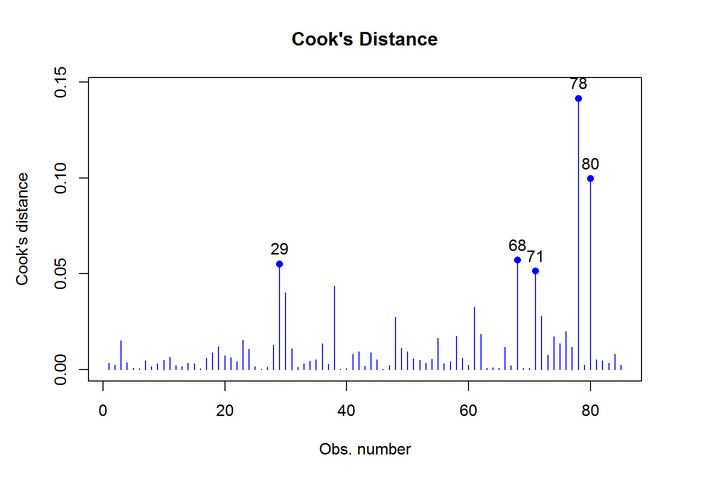
\includegraphics[width=0.7\linewidth]{images/CooksDistancePlot-JS-Roy}
	\caption{}
	\label{fig:CooksDistancePlot-JS-Roy}
\end{figure}

\begin{figure}[h!]
	\centering
	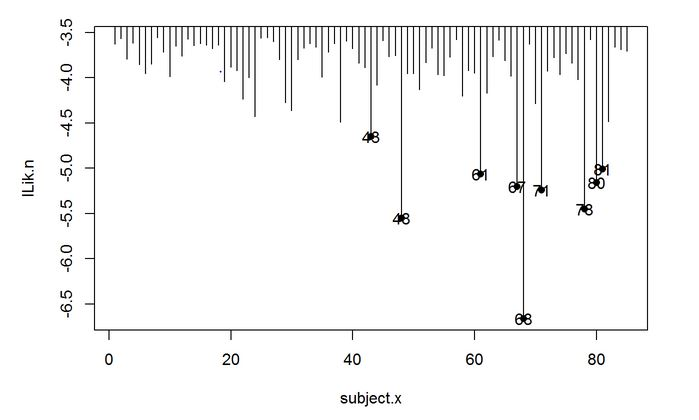
\includegraphics[width=0.7\linewidth]{images/LogLik-JS-Roy}
	\caption{}
	\label{fig:LogLik-JS-Roy}
\end{figure}

As the model is structurally different from the models discussed in the earlier sections, Residual analysis will be briefly revisited.
\begin{figure}[h!]
	\centering
	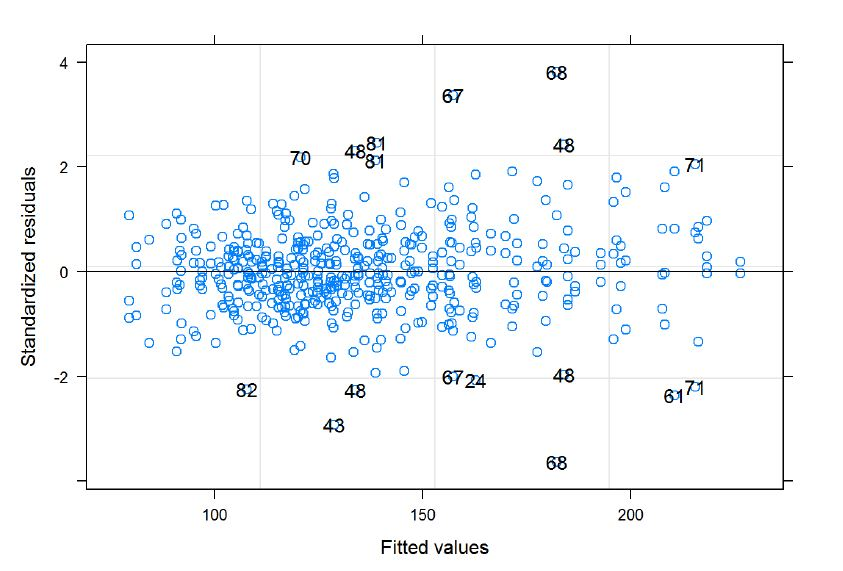
\includegraphics[width=0.7\linewidth]{images/Residuals-JS-Roy}
	\caption{}
	\label{fig:Residuals-JS-Roy}
\end{figure}

\section{Case Deletion Diagnostics for Variance Ratios}
%- H Case Deletion Diagnostics 

\citet{schabenberger} advises on the use of deletion diagnostics for variance components of an LME model.

Taking the core principals of his methods, and applying them to the Method Comparison problem, case deletion diagnostics are used on the variance components of the Roy model., specifically the ratio of between subject variances and the within subject covariances respecitvely.


\[ \mbox{BSVR} = \frac{\sigma^2_2}{\sigma^2_2} \phantom{makespace}  \mbox{WSVR} = \frac{d^2_2}{d^2_2} \]

These variance ratios are re-computed for each case removed, and may be analysed seperately or jointly for outliers. 

%============================================== %
\subsection{Methods for Identifying Outliers}
The Grubbs' Test for Outliers is a commonly used technique for assessing outlier in a univariate data set, of which there are several variants. The first variant of Grubb's test is used to detect if the sample dataset contains one outlier, statistically different than
the other values. The test statistic is based by calculating score of this outlier $G$ (outlier minus mean and divided
by sd) and comparing it to appropriate critical values. Alternative method is calculating ratio of
variances of two datasets - full dataset and dataset without outlier. 
%The obtained value called U is bound with G by simple formula.
The second variant is used to check if lowest and highest value are two outliers on opposite tails of sample. It is based on calculation of ratio of range to standard deviation of the sample.

The third variant calculates ratio of variance of full sample and sample without two extreme observations.
It is used to detect if dataset contains two outliers on the same tail.

As there may be several outliers present, the Grubbs test is not practical. However an indication that a point being beyond the fences according to Tukey's 
specification for boxplots, ( i.e. greater than $Q_3 +1.5 \mbox{IQR}$ or less than $Q_1 - 1.5 \mbox{IQR}$), will suffice.

\subsection{Mahalanbis Distance}
Bivariate Analyses may be applied jointly to the both sets of data sets, e.g Mahalanobis distances.

The WSVR values are plotted against the corresponding BSVR values. Confidence Ellipses can be superimposed over the plot with minimal effort. Two ellipses are generated by this technique, a 50 \% and 97.5\% confidence ellipse respectively. Outlying cases are idenified by the plot. Subject 68 is evident

The subjects were ranked by Mahalanobis distance, with the top 10 being presented in the following table. Both sets of ratio are addtionally expressed as a ratio of the full model variance ratios. 
\begin{center}
	\begin{tabular}{|c|c|c|c|c|c|}
		\hline
		Subject (u) &  MD & WSVR$_{(u)}$ & WSVR (\%) & BSVR$_{(u)}$   & BSVR (\%)     \\ \hline \hline
		68 & 44.7284   & 1.3615  & 0.9132   & 1.0353  & 0.9849 \\ \hline
		30 & 16.7228   & 1.5045  & 1.0092   & 1.1024  & 1.0487 \\ \hline
		71 & 11.5887   & 1.5210  & 1.0202   & 1.0932  & 1.0400 \\ \hline
		80 & 11.0326   & 1.4796  & 0.9925   & 1.0114  & 0.9621 \\ \hline 
		38 & 10.3671   & 1.5011  & 1.0069   & 1.0917  & 1.0385 \\ \hline 
		67 & 10.1940   & 1.4308  & 0.9598   & 1.0514  & 1.0002 \\ \hline
		43  & 7.6932   & 1.4385  & 0.9649   & 1.0511  & 0.9999 \\ \hline
		72  & 4.7350   & 1.4900  & 0.9995   & 1.0262  & 0.9762 \\ \hline
		48  & 4.4321   & 1.4950  & 1.0028   & 1.0280  & 0.9779 \\ \hline
		29  & 4.3005   & 1.4910  & 1.0001   & 1.0769  & 1.0244 \\ \hline
	\end{tabular} 
\end{center}
From this table one may conclude that subjects 72, 48 and 29 are not particularly influential. Interestingly Subject 78, which was noticeable in the case deletion diagnostics for fixed effects, does not feature in this table.

\begin{figure}[h!]
	\centering
	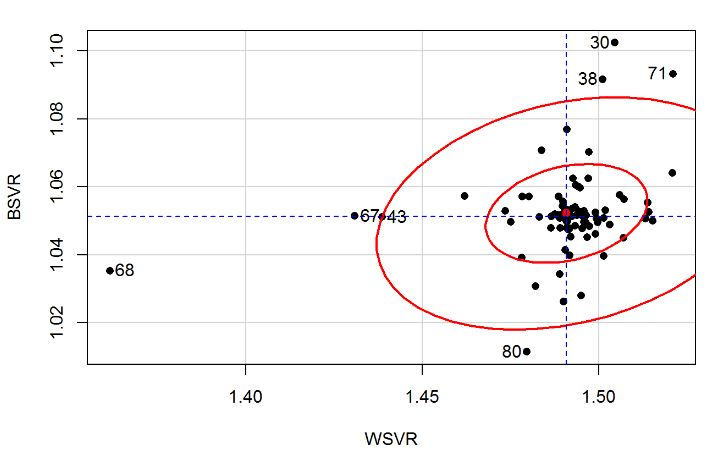
\includegraphics[width=0.9\linewidth]{08-plot1}
	\caption{}
	\label{fig:08-plot1}
\end{figure}



%===========================================================================%

\subsection{Variance Ratios}
The approach proposed by Roy deals with the question of agreement, and indeed interchangeability, as developed by Bland and Altman’s corpus of work.  In the view of Dunn, a question relevant to many practitioners is which of the two methods is more precise.
The relationship between precision and the within-item and between-item variability must be established. Roy establishes the equivalence of repeatability and within-item variability, and hence precision.  The method with the smaller within-item variability can be deemed to be the more precise.

A useful approach is to compute the confidence intervals for the ratio of within-item standard deviations (equivalent to the ratio of repeatability coefficients), which can be interpreted in the usual manner.  

In fact, the ratio of within-item standard deviations, with the attendant confidence interval,  can be determined using a single R command: \texttt{intervals()}.

Pinheiro and Bates (pg 93-95) give a description of how confidence intervals for the variance components are computed. Furthermore a complete set of confidence intervals can be computed to complement the variance component estimates. 

What is required is the computation of the variance ratios of within-item and between-item standard deviations.  

A naïve approach would be to compute the variance ratios by relevant F distribution quantiles. However, the question arises as to the appropriate degrees of freedom.
Limits of agreement are easily computable using the LME framework. While we will not be considering this analysis, a demonstration will be provided in the example.






%\subsection*{5. Using Roy's Test to Identify cause of Lack of agreement}
%
%Barnhart specifies three conditions for method of measurement that are required for two methods of measurement to be considered in agreement.
%
%\begin{itemize}
%	\item[(i)] No Significant Inter-method bias
%	\item[(ii)] No significant Difference in Within-Subject Variance
%	\item[(iii)] No significant Difference in Within-Subject Variance 
%\end{itemize}
%
%
%Roy(2009) demonstrates a LME model specification, and a series of tests that look at each of these agreement criteria individually. If two methods of measuement lack agreement, the specific reason or reasons for this lack of agreement can be identified.
%
%
%Roy proposes an LME model with Kronecker product covariance structure in a doubly multivariate setup. Response for $i$th subject can be written as
%\[ y_i = \beta_0 + \beta_1x_{i1} + \beta_2x_{i2} + b_{1i}z_{i1}  + b_{2i}z_{i2} + \epsilon_i \]
%\begin{itemize}
%	\item $\beta_1$ and $\beta_2$ are fixed effects corresponding to both methods. ($\beta_0$ is the intercept.)
%	\item $b_{1i}$ and $b_{2i}$ are random effects corresponding to both methods.
%\end{itemize}
%
%Overall variability between the two methods ($\Omega$) is sum of between-subject ($D$) and within-subject variability ($\Sigma$),
%\[
%\mbox{Block } \boldsymbol{\Omega}_i = \left[ \begin{array}{cc} d^2_1 & d_{12}\\ d_{12} & d^2_2\\ \end{array} \right]
%+ \left[\begin{array}{cc} \sigma^2_1 & \sigma_{12}\\ \sigma_{12} & \sigma^2_2\\ \end{array}\right].
%\]
%============================================== %
%- F:

\chapter{Cook's Distance}
Application of Cooks Distances are limited by compuation tractability.


Application of case-deletion diagnostics offer some interested for Method Comparison Studies


Care must be given when interpreting these plots. For example the position of case 68 on the BSVR indicates that that
case 68 

A similar plot may be constructed using the

Any diagnostic plot may constructed using Overall variability and intermethod bias.



\section{Cook's Distance}
\citet{Christensen} develops \index{case deletion diagnostics} case deletion diagnostics, in particular the equivalent of \index{Cook's distance} Cook's distance, a well-known metric, for diagnosing influential observations when estimating the fixed effect parameters and variance components. Deletion diagnostics provide a means of assessing the influence of an observation (or groups of observations) on inference on the estimated parameters of LME models. 
%We shall provide a fuller discussion of Cook's distance in due course.
Cook's Distance is a good measure of the influence of an observation that is a measure of aggregate impact of each observation on the group of regression coefficients, as well as the group of fitted values.
%Cook's Distance is proportional to the sum of the squared differences between predictions made with all observations in the analysis and predictions made leaving out the observation in question. 
If the predictions are the same with or without the observation in question, then the observation has no influence on the regression model. If the predictions differ greatly when the observation is not included in the analysis, then the observation is influential.

%======================================================================================= %



%======================================================================================= %
\subsubsection{Cook's Distance for Blood Data}
\begin{figure}[h!]
	\centering
	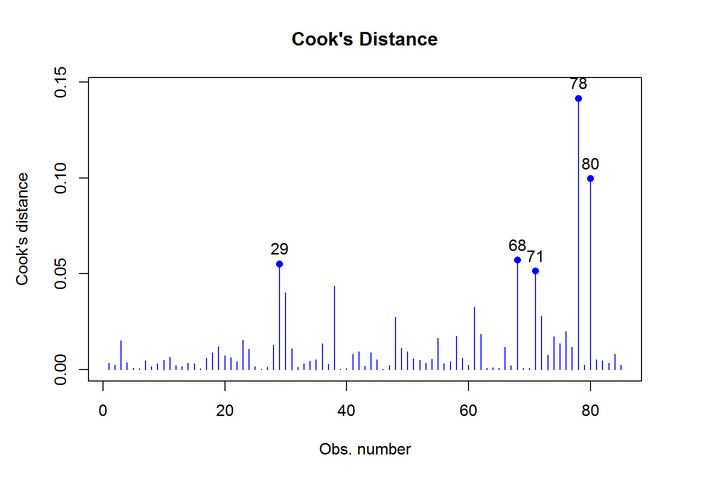
\includegraphics[width=0.9\linewidth]{images/CooksDistancePlot-JS-Roy}
	%	\caption{}
	%	\label{fig:CooksDistancePlot-JS-Roy}
\end{figure}

%============================================================================= %

% Hence the name deletion diagnostics and case-deletion diagnostics. 
\subsection{Cook's Distance}%1.9.2
\index{Cook's distance} Cook's $D$ statistics (i.e. colloquially Cook's Distance) is a measure of the influence of observations in subset $U$ on a vector of parameter estimates \citep{cook77}.

\[ \delta_{(U)} = \hat{\beta} - \hat{\beta}_{(U)}\]

If V is known, Cook's D can be calibrated according to a chi-square distribution with degrees of freedom equal to the rank of $\boldsymbol{X}$ \citep{cpj92}.


For LME models, Cook's distance can be extended to model influence diagnostics by defining.

%\[ C_{\beta i} = {(\hat{\beta} - \hat{\beta}_{[i]})^{T}(\boldsymbol{X}^{\prime}\boldsymbol{V}^{-1}\boldsymbol{X}) (\hat{\beta} - \hat{\beta}_{[i]}) \over p}\]





\subsection{Cooks distance- Predict means thing here}

Further to previous work, this section revisits case-deletion and residual diagnostics, and explores how approaches devised by  Galecki \& Burzykowski (2013) can be used to appraise Roy's model. These authors specifically look at Cook's Distances and Likelihood Distances.
For the Roy Model, Cook's Distances may also be generated using the \textbf{\textit{predictmeans}}

\subsection{Cook's Distance for Blood Data}



\begin{figure}[h!]
	\centering
	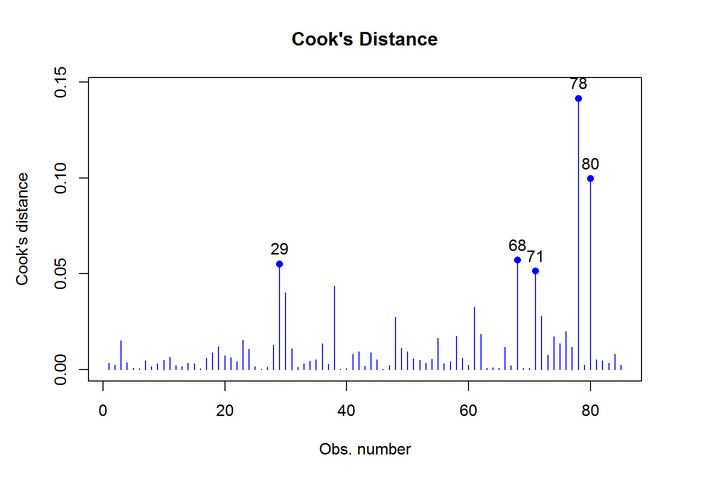
\includegraphics[width=0.7\linewidth]{images/CooksDistancePlot-JS-Roy}
	\caption{}
	\label{fig:CooksDistancePlot-JS-Roy}
\end{figure}

\begin{figure}[h!]
	\centering
	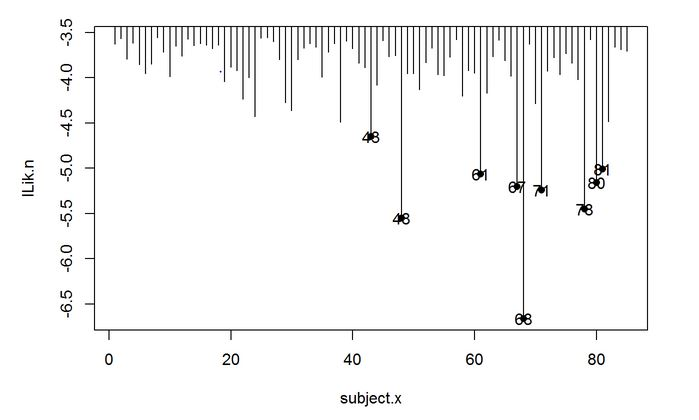
\includegraphics[width=0.7\linewidth]{images/LogLik-JS-Roy}
	\caption{}
	\label{fig:LogLik-JS-Roy}
\end{figure}

As the model is structurally different from the models discussed in the earlier sections, Residual analysis will be briefly revisited.
\begin{figure}[h!]
	\centering
	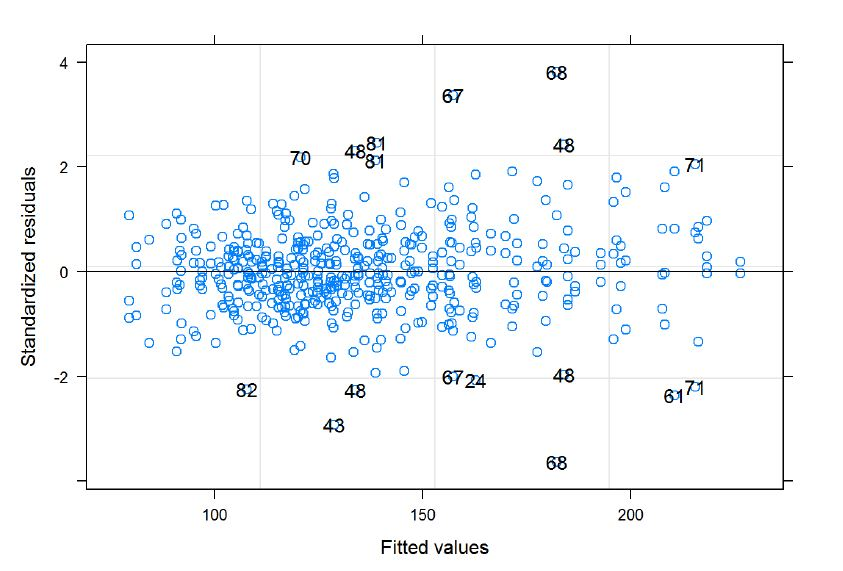
\includegraphics[width=0.7\linewidth]{images/Residuals-JS-Roy}
	\caption{}
	\label{fig:Residuals-JS-Roy}
\end{figure}


Cook's Distance is a model diagnostic measure of an observation that is a measure of aggregate impact of each observation on the group of regression coefficients. Observations, or sets of observations, that have high Cook's distance usually have high resdiauls. We will revisit Cook's distance fully in due cource.

Cook's Distance is a good measure of the influence of an observation that is a measure of aggregate impact of each observation on the group of regression coefficients, as well as the group of fitted values.

The \texttt{CookD} fucntion , from the predictmeans R package, produces Cook’s distance plots for an LME model 
(predictmeans)



\begin{framed}
	\begin{verbatim}
	library(predictMeans)
	CookD(model, group=method, plot=TRUE, idn=5, newwd=FALSE)
	\end{verbatim}
\end{framed}


\begin{verbatim}
## Cook's Distance

\end{verbatim}

The particular cases that we will omit for the subsequent analysis are subjects 68,78 and 80.

\subsection{Reduced Data Set}
It is important to determine if a specific group of cases or subjects give rise to the lack of agreement in the methods. If one were to examine fitted model if these cases were removed.

\begin{framed}
	\begin{verbatim}
	
	blood.red <- blood[!(blood$subject %in% c(68,78,80)),]
	dim(blood.red)
	# 27 observations should be removed.
	
	blood.NLME.red <-lme(BP ~ method-1 , random=~1|subject,data = blood.red)
	plot(blood.NLME.red, resid(., type = "p") ~ fitted(.) | method, abline = 0, id=.05)
	\end{verbatim}
\end{framed}

In this instance, we conclude that there is a systemic diagreement between method S and the other two methods, and that lack of agreement can not be sourced to a handful of cases.
\begin{figure}[h!]
	\centering
	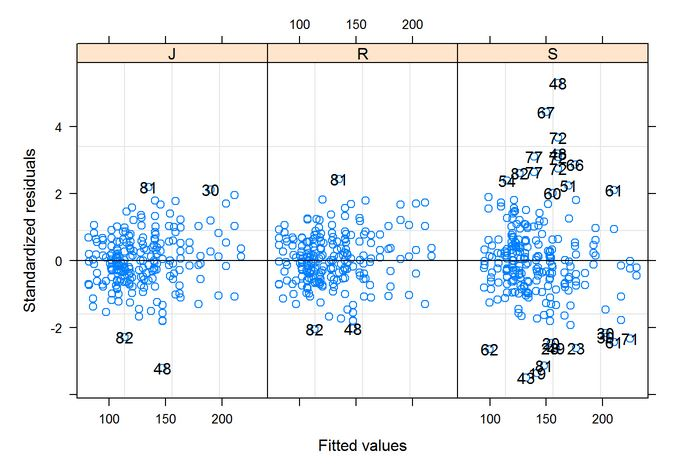
\includegraphics[width=0.7\linewidth]{images/bloodnlmeResidPlot2B}
\end{figure}


\newpage





\subsection{Cook's Distance for LMEs} %1.10



% %- OLS
\index{Cook's Distance} Cooks Distance ($D_{i}$) is a well known diagnostic technique used in classical linear models, that functions an overall measure of the combined impact of the $i$th case of all estimated regression coefficients. It uses the same structure for measuring the combined impact of the differences in the estimated regression coefficients when the $i$th case is deleted. $D_{(i)}$ can be calculated without fitting a new regression coefficient each time an observation is deleted. Importantly, $D_{(i)}$ can be calculated without fitting a new regression coefficient each time an observation is deleted.

\index{Cook's distance} Cook's $D$ statistics (i.e. colloquially Cook's Distance) is a measure of the influence of observations in subset $U$ on a vector of parameter estimates \citep{cook77}.

\[ \delta_{(U)} = \hat{\beta} - \hat{\beta}_{(U)}\]

If V is known, Cook's D can be calibrated according to a chi-square distribution with degrees of freedom equal to the rank of $\boldsymbol{X}$ \citep{cpj92}. (\textbf{State V and X})


% %- Interpretation
Cook's distance can be used in several ways: to indicate data points that are particularly worth checking for validity; to indicate regions of the design space where it would be good to be able to obtain more data points. 
Large values for Cook's distance indicate observations for special attention. 

Use of threshold value for Cook's Distance is discouraged (\textbf{cite: JohnFox}). However, informal heuristics do exist for OLS models; Obervations for which Cook's distance is higher than 1 are to be considered as influential. Alternatively there is an informal threshold of $4/N$ or $4/(N−k−1)$, where N is the number of observations and k the number of explanatory variables.

% Interpretation
% http://stats.stackexchange.com/questions/22161/how-to-read-cooks-distance-plots %

% Fox, John. (1991). Regression Diagnostics: An Introduction. Sage Publications.

\textbf{cite: JohnFox} advises the use of diagnostic plotting and to examine in closer details the points with "\textit{values of D that are substantially larger than the rest}", and that thresholds should just be used to enhance graphical displays.


The effect on the precision of estimates is separate from the effect on the point estimates. Data points that have a small \index{Cook's distance}Cook's distance, for example, can still greatly affect hypothesis tests and confidence intervals, if their  influence on the precision of the estimates is large.

%
%\subsubsection{Interpretation}
%Specifically $D_i$ can be interpreted as the distance one's estimates move within the confidence ellipsoid that represents a region of plausible values for the parameters.[clarification needed] This is shown by an alternative but equivalent representation of Cook's distance in terms of changes to the estimates of the regression parameters between the cases where the particular observation is either included or excluded from the regression analysis.
%
%================================================ %
% %- Exention to LMEs
\citet{Christensen} would later adapt the \index{Cook's distance}Cook's Distance measure for the analysis of LME models. For LME models, two formulations exist; a \index{Cook's distance}Cook's distance that examines the change in fixed fixed parameter estimates, and another that examines the change in random effects parameter estimates. The outcome of either Cook's distance is a scaled change in either $\beta$ or $\theta$.

For LME models, Cook's distance can be extended to model influence diagnostics by defining.

\[ CD_{\beta i} = {(\hat{\beta} - \hat{\beta}_{[i]})^{T}(\boldsymbol{X}^{\prime}\boldsymbol{V}^{-1}\boldsymbol{X}) (\hat{\beta} - \hat{\beta}_{[i]}) \over p}\]

It is also desirable to measure the influence of the case deletions on the covariance matrix of $\hat{\beta}$.

\subsection{Taxonomy of Cook's Distances for LMEs}
\citet{schabenberger} discusses a taxonomy of Cook's distance when applied to LME models. \begin{itemize}
	\item For variance components $\gamma$: $CD(\gamma)_i$,
	\item For fixed effect parameters $\beta$: $CD(\beta)_i$,
	\item For random effect parameters $\boldsymbol{u}$: $CD(u)_i$,
	\item For linear functions of $\hat{beta}$: $CD(\psi)_i$
\end{itemize}			
%============================================================================= %


It is also desirable to measure the influence of the case deletions on the covariance matrix of $\hat{\beta}$.
% % - Fixed Effects Parameter		

For fixed effects parameter estimates in LME models, the \index{Cook's distance} Cook's distance can be extended to measure influence on these fixed effects.

\[
\mbox{CD}_{i}(\beta) = \frac{(c_{ii} - r_{ii}) \times t^2_{i}}{r_{ii} \times p}
\]


For fixed effects parameter estimates in LME models, the \index{Cook's distance} Cook's distance can be extended to measure influence on these fixed effects.

\[
\mbox{CD}_{i}(\beta) = \frac{(c_{ii} - r_{ii}) \times t^2_{i}}{r_{ii} \times p}
\]

For random effect estimates, the \index{Cook's distance} Cook's distance is

\[
\mbox{CD}_{i}(b) = g{\prime}_{(i)} (I_{r} + \mbox{var}(\hat{b})D)^{-2}\mbox{var}(\hat{b})g_{(i)}.
\]
Large values for Cook's distance indicate observations for special attention.

A large value for $CD(u)_i$ indicates that the $i-$th observation is influential in predicting random effects.
For linear functions, $CD(\psi)_i$ does not have to be calculated unless $CD(\beta)_i$ is large.
%===================================================== %


\subsection{Cook's Distance}

Diagnostic tool for variance components
\[ C_{\theta i} =(\hat(\theta)_{[i]} - \hat(\theta))^{T}\mbox{cov}( \hat(\theta))^{-1}(\hat(\theta)_{[i]} - \hat(\theta))\]

\begin{description}
	\item[Random Effects]	
	A large value for $CD(u)_i$ indicates that the $i-$th observation is influential in predicting random effects.
	\item[linear functions]
	$CD(\psi)_i$ does not have to be calculated unless $CD(\beta)_i$ is large.
\end{description}






\subsubsection{linear functions}

$CD(\psi)_i$ does not have to be calculated unless $CD(\beta)_i$ is large.



%-------------------------------------------------------------------------------------------------------------------------------------%







\chapter{Using DFBETAs from LME Models to Assess Agreement}


\citet{schabenberger} examines the use and implementation of influence measures in LME models.

Influence is understood to be the ability of a single or multiple data points, through their presences or absence in the data, to alter important aspects of the analysis, yield qualitatively 	different inferences, or violate assumptions of the statistical
model \citep{schabenberger}.

Outliers are the most noteworthy data points in an analysis, and an objective of influence analysis is how influential they are,
and the manner in which they are influential.

\citet{schabenberger} describes a simple procedure for quantifying influence.
\begin{itemize}
	\item Firstly a model should be fitted to the data, and
	estimates of the parameters should be obtained.
	\item The second step is that either single or multiple data points, specifically outliers,
	should be omitted from the analysis, with the original parameter
	estimates being updated.
	\item  The final step of the procedure is comparing the 	sets of estimates computed from the entire and reduced data sets
	to determine whether the absence of observations changed the
	analysis.
\end{itemize}
This is known as `\textit{leave one out} or \texttt{leave k
	out' analysis}.






\section*{Case Deletion Diagnostics for LME Data: Cooks Distance, DFBetas}
In this section we introduce influence analysis and case deletion diagnosics. A full overview of the topic will be provided although there are specific tools that are particularly useful in the case of MCS problems: specifically the Cook's Distance and the DFBeta.

A discussion of how leave-k-out diagnostics would work in the context of MCS problems is required. There are several scenaros. Suppose we have two methods of measurement X and Y, each with three measurements for a specific case: $(x_1,x_2,x_3,y_1,y_2,y_3)$

\begin{itemize}
	\item Leave One Out - one observation is omitted (e.g. $x_1$)
	\item Leave Pair Out - one pair of observation  is omitted (e.g. $x_1$ and $y_1$)
	\item Leave Case (or Subject) Out - All observations associated with a particular case or subject are omitted. (e.g. $\{x_1,x_2,x_3,y_1,y_2,y_3\}$)
\end{itemize}
Other metrics, such as the likelihood distance, will also be introduced, and revisited in a later section.

\section{Application of DFBETAs in MCS Analysis}

When in an MCS study. DFBetas can be used as a proxy measurement, allowing simple techniques to be used for assessing agreement.

Suppose an LME model was formulated to model agreement for various (i.e. 2 or more) methods of measurement, with replicate measurements. If the methods are to be agreement, the DFBetas for each case would be the same for both methods.\textbf{As such, agreement between any two methods can be determined by a simple scatterplot of the DFBetas. If the points align along the line of equality, then both methods can be said to be in agreement.}

%Cook's Distance can be used to identify and rank cases, in terms of influence.
For the model fitted to the blood data with the lme4 R package, the results tabulated below can be produced. All 85 subjects are ranked by Cook's Distance (with only the top 6 being presented here). The remaining columns are the DFBeta for each of the fixed effects, for each of the 85 subject.
\begin{center}
	\begin{tabular}{|c|c|c|c|c|} \hline
		Subject &    Cook's D  &    methodJ  &   methodR  & methodS \\ \hline \hline
		78 & 0.61557407 & -0.02934556 & -0.03387780 & 0.2954937  \\ \hline
		80 & 0.41590973 & -0.06305026 & -0.06515241 & 0.2123881  \\ \hline
		68 & 0.22536651 & -0.05334867 & -0.05062375 & 0.1555187  \\ \hline
		72 & 0.09348500  & 0.02388626  & 0.02419887 & 0.1617474  \\ \hline
		48 & 0.08706988  & 0.02147541  & 0.03145273 & 0.1581591  \\ \hline
		30 & 0.07118415  & 0.26925807  & 0.26215970 & 0.1581569  \\ \hline
	\end{tabular} 
\end{center}
\newpage
\begin{figure}[h!]
	\centering
	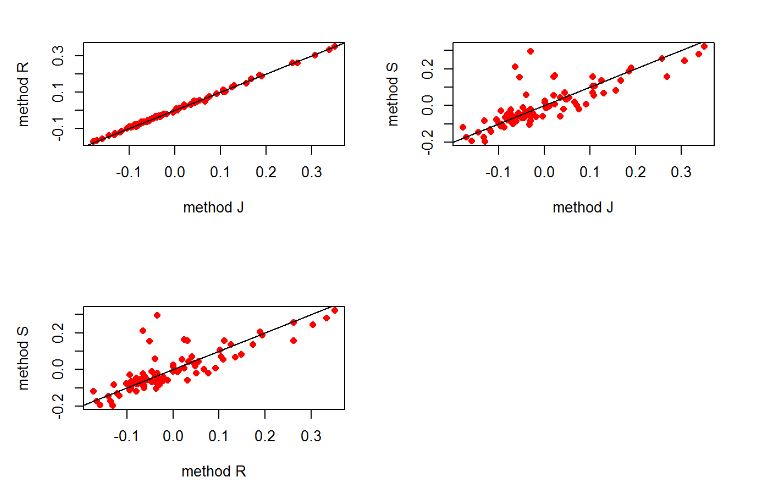
\includegraphics[width=0.9\linewidth]{images/04-DFbetaplots}
	% \caption{}
	% \label{fig:04-DFbetaplots}
\end{figure}

In the first of the three plots (\textit{Top Right}), strong agreement between method J and method R is indicated. The other plots indicate lack of agreement of methods J and R with method S.



If lack of agreement is indicated, a subsequent analysis using a technique proposed by Roy(2009) can be used to identify the specific cause for this lack of agreement (see next section).
\newpage

The Pearson Correlation coefficient of the DFBetas can be used in conjection with this analysis. A high correlation confirms good agreement. No threshold value for agreement is suggested, and analysts are advised to perform model diagnostics regardless of the correlation coeffient. 


The Bonferroni Outlier Test and Cook's Distance values can be used to identify unusual cases, when the relationship between sets of dfbeta is modelled as a (classical) linear model. In this model, the covariates should be homoskedastic. A test for non-constant variance may be used to verify this. These diagnostic procedures are implementable using the \textbf{\textit{car}} R package.


Deming Regression can be used to verify the line of equality. Significance test for Deming regression estimates are not available, but 95\% bootstrap confidence intervals for the slope estimate and intercept estimates can be computed. 


Additionally a mean difference plot can be used to identify outliers. This mean-difference plot differs from the Bland-Altman plot in that the plot is denominated in terms of dfbeta values, and not in measurement units.

If lack of agreement is indicated between methods of measurement, use of Roy's Testing is advised (This is the subject of the next section).
\begin{figure}[h1]
	\centering
	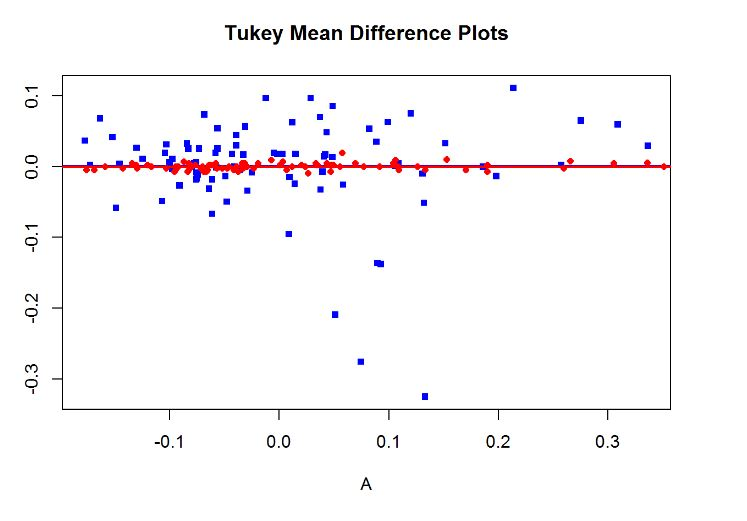
\includegraphics[width=0.7\linewidth]{images/04-TMDplot}
	
\end{figure}
\newpage



\chapter{Other Stuff}

\section{Diagnostic Tools for the nlme package}


With the nlme package, the generic function \texttt{lme()} fits a linear mixed-effects model in the formulation described in Laird and Ware (1982) but allowing for nested random effects. 

The within-group errors are allowed to be correlated and/or have unequal variances, which is very important in fitting the models for Roy's Tests

The nlme package has a limited set of diagnostic tools that can be used to assess the model fit. A review of the package manual is sufficient to get a sense of the package's capability in that regard.




\section{Influence() - Description}
\texttt{influence()} is the workhorse function of the \texttt{influence.ME} package. 


Based on a priorly estimated mixed effects regression model (estimated using lme4), the \texttt{influence()} function iteratively 

modifies the mixed effects model to neutralize the effect a grouped set of data has on the parameters, and which 

returns returns the fixed parameters of these iteratively modified models. 

These are used to compute measures of influential data.




%\subsection*{Usage}
%\begin{framed}
%	\begin{verbatim}
%	
%	influence(model, group=NULL, select=NULL, obs=FALSE, 
%	gf="single", count = FALSE, delete=TRUE, ...)
%	\
%	\end{verbatim}
%\end{framed}
%
%
%The \texttt{influence()} function was known as the \texttt{estex()} command in previous versions of the influence.ME pacakge
%===========================================================================%
%- http://support.sas.com/documentation/cdl/en/statug/63347/HTML/default/statug_reg_sect040.htm









\section{Leave-One-Out Diagnostics with \texttt{lmeU}}
Galecki et al discuss the matter of LME influence diagnostics in their book, although not into great detail.


The command \texttt{lmeU} fits a model with a particular subject removed. The identifier of the subject to be removed is passed as the only argument

A plot ofthe per-observation diagnostics individual subject log-likelihood contributions can be rendered.

%% Page 503 Galecki

\section{Partitioning Matrices} %1.14.2
Without loss of generality, matrices can be partitioned as if the $i-$th omitted observation is the first row; i.e. $i=1$.


\section{Permutation Test, Power Tests and Missing Data }

This section explores topics such as dependent variable simulation and power analysis, introduced by Galecki \& Burzykowski (2013), and implementable with their \textbf{\textit{nlmeU}} \texttt{R} package.
Using the \textbf{\textit{predictmeans}} \texttt{R} package, it is possible to perform permutation t-tests for coefficients of (fixed) effects and permutation F-tests.

The matter of missing data has not been commonly encountered in either Method Comparison Studies or Linear Mixed Effects Modelling. However Roy (2009) deals with the relevant assumptions regrading missing data. Galecki \& Burzykowski (2013) approaches the subject of missing data in LME Modelling. The \textbf{\textit{nlmeU}} package includes the \texttt{patMiss} function, which ``\textit{allows to compactly present pattern of missing data in a given vector/matrix/data
	frame or combination of thereof}".




\section{The \texttt{logLik} Function}
\texttt{logLik.lme} returns the log-likelihood value of the linear mixed-effects model represented by object evaluated at the estimated coefficients. It is also possible to determine the restricted log-likelihood, if relevant, using this function. For the Blood Data Example,  the loglikelihood of the JS.roy1 model can be computed as follows.
\begin{framed}
	\begin{verbatim}
	> logLik(JS.roy1)
	'log Lik.' -2030.736 (df=8)
	\end{verbatim}
\end{framed}
\bibliographystyle{chicago}
\bibliography{DB-txfrbib}


\end{document}